% !TEX root = ../../main.tex

\section{Approximation de la partie linéaire}
\label{s3:approx}

L'obtention, à l'aide d'un logiciel de calcul formel, de l'exponentielle de la partie linéaire n'est pas toujours envisageable. Il est possible de recourir à une méthode d'approximation pour obtenir une formulation formelle de celle-ci qui sera possible d'utiliser pour l'écriture du code de simulation. On s'intéressera dans cette section à la partie linéaire $L$ définie par :
$$
  L = \begin{pmatrix}
    0   & -B_0 & 0          &  0          &  \Omega_{pe}^2 & 0             & 0 \\
    B_0 &  0   & 0          &  0          &  0             & \Omega_{pe}^2 & 0 \\
    0   &  0   & 0          &  0          &  0             & \partial_z    & 0 \\
    0   &  0   & 0          &  0          & -\partial_z    & 0             & 0 \\
   -1   &  0   & 0          & -\partial_z &  0             & 0             & 0 \\
    0   & -1   & \partial_z &  0          &  0             & 0             & 0 \\
    0   &  0   & 0          &  0          &  0             & 0             & -v_z\partial_z \\
  \end{pmatrix}
$$
où on rappelle que $\Omega_{pe}=2$. Cette matrice est de la forme :
$$
  L = \begin{pmatrix}
    A & 0 \\
    0 & -v_z\partial_z
  \end{pmatrix}
$$
matrice diagonale par blocs, dont seul le bloc $A$ pose problème pour calculer formellement l'exponentielle. Ainsi on s'intéressera surtout à la sous-matrice $A$ obtenue après une transformée de Fourier en $z$ du système :
$$
  A = \begin{pmatrix}
    0 & -1 & 0  &  0  &  \Omega_{pe}^2  & 0             \\
    1 &  0 & 0  &  0  &  0              & \Omega_{pe}^2 \\
    0 &  0 & 0  &  0  &  0              & ik            \\
    0 &  0 & 0  &  0  & -ik             & 0             \\
   -1 &  0 & 0  & -ik &  0              & 0             \\
    0 & -1 & ik &  0  &  0              & 0             \\
  \end{pmatrix}
$$
Par abus de notation, nous noterons $A_0$, la matrice $A$ pour $k=0$, ce qui revient à une partie linéaire sans les équations de Maxwell, ceci sera utile lors de la comparaison des résultats entre les méthodes.

La matrice $A$ est telle que toutes ses valeurs propres sont imaginaires pures, $\texttt{sp}(A)\subset i\mathbb{R}$. De plus, $A$ est presque anti-hermitienne, on peut trouver une matrice de passage $\Omega$ permettant de transformer notre matrice $A$ en une matrice anti-hermitienne :
$$
  \Omega = 
  \begin{pmatrix}
    \dmat[0]{\Omega_{pe}^{-1/2},\Omega_{pe}^{-1/2},\Omega_{pe}^{1/2},\Omega_{pe}^{1/2},\Omega_{pe}^{1/2},\Omega_{pe}^{1/2}}
  \end{pmatrix},
$$
où $\Omega$ est obtenu avec les mêmes stratégies qu'un symétriseur. On a $H=\Omega A \Omega^{-1}$ anti-hermitienne. Le spectre de $H$ est imaginaire pur, et $H$ est diagonalisable dans une base orthonormale, c'est-à-dire :
$$
  \exists Q \in GL_6(\mathbb{C}) / H = QDQ^{-1}, \|Q\|=1
$$
où $D$ est une matrice diagonale des valeurs propres de $H$. Ce qui nous permet de déterminer que les valeurs propres de l'exponentielle de $H$ sont sur le cercle unitaire, en effet :
$$
  \forall t\in\mathbb{R}, e^{tH} = Qe^{tD}Q^{-1}.
$$
Et on a, de même pour la matrice $A$, des valeurs propres distribuées sur le cercle unité, avec la matrice de passage $\Omega Q$, comme l'illustre la figure~\ref{fig:evexpAk}, où les valeurs propres de $A$ sont calculées numériquement pour différents modes de Fourier.

\begin{figure}
  \centering
  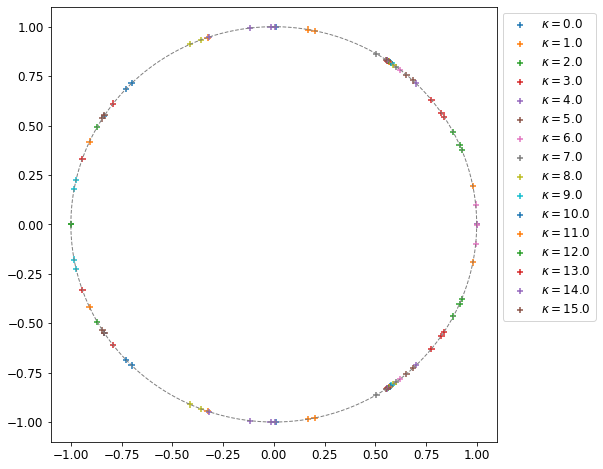
\includegraphics[width=0.5\textwidth]{\localPath/figures/evexpAk.png}
  \caption{Valeurs propres de $e^{A}$ pour différentes fréquences $\kappa\in[\![0,15]\!]$. Les valeurs propres des modes de Fourier négatifs, sont obtenues par parité.}
  \label{fig:evexpAk}
\end{figure}

\subsection{Troncature de la série de Taylor}
%--------------------------------------------------------------------

Un manière classique de définir la fonction exponentielle est par sa série de Taylor, ainsi on définit $e^{tA}$ par :
$$
  e^{tA} = \sum_{n=0}^\infty \frac{t^nA^n}{n!}.
$$
Une troncature d'ordre suffisamment élevé permet d'obtenir une approximation de l'exponentielle $e^{tA}$ à un ordre plus élevé que la méthode LRK($s$,$n$) où elle sera utilisé garanti que l'erreur de troncature reste inférieur à $n$, l'ordre de la méthode en temps. On définit la troncature de la série de Taylor à l'ordre $m$ par :
$$
  T_m(A) = \sum_{k=0}^m \frac{A^k}{k!}.
$$

Nous savons que les valeurs propres de $e^{A}$ sont sur le cercle unité, préserver cette propriété permet d'assurer la stabilité du schéma. Nous regardons donc les valeurs propres de $T_5(A)$, pour les modes de Fourier $\kappa\in[\![0,15]\!]$ sur la figure~\ref{fig:ev:T5}. On remarque que le module des valeurs propres à 1 n'est pas préservé.

\begin{figure}
  \begin{subfigure}{.5\textwidth}
    \centering
    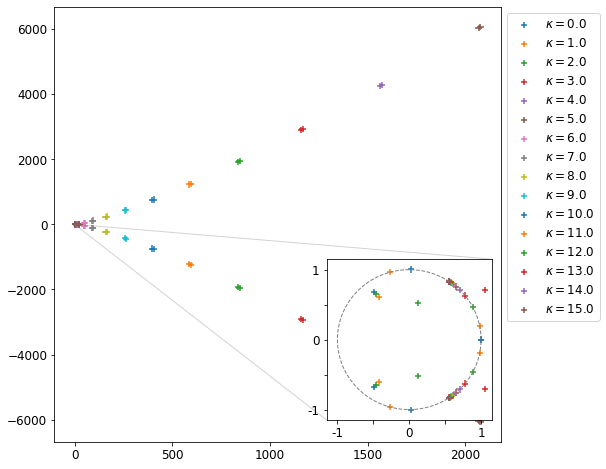
\includegraphics[width=\textwidth]{\localPath/figures/ev_T5.png}
    \caption{Valeurs propres de $T_5(A)$ pour différentes fréquences $\kappa\in[\![0,15]\!]$.}
    \label{fig:ev:T5}
  \end{subfigure}
  \begin{subfigure}{.5\textwidth}
    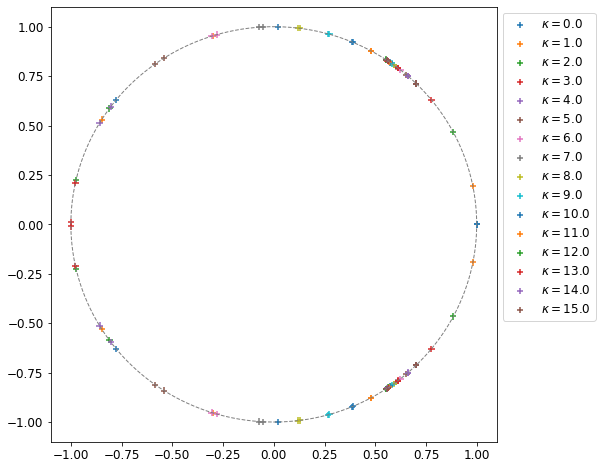
\includegraphics[width=\textwidth]{\localPath/figures/ev_P22.png}
    \caption{Valeurs propres de $P_{2,2}(A)$ pour différentes fréquences $\kappa\in[\![0,15]\!]$.}
    \label{fig:ev:P22}
  \end{subfigure}
  \caption{Valeurs propres de l'approximation de l'exponentielle de $A$ pour différentes fréquences $\kappa\in[\![0,15]\!]$. Les valeurs propres des modes de Fourier négatifs sont obtenues par paritée. Les méthodes d'approximation de l'exponentielle de $A$ sont la troncature de Taylor d'ordre 5 $T_5(A)$ (à gauche) et l'approximant de Padé d'ordre $(2,2)$ $P_{2,2}(A)$ (à droite).}
\end{figure}

On peut regarder, pour différentes valeurs de $m$, l'erreur de troncature faite en norme matricielle pour 2 modes de Fourier $\kappa=2$ et $15$. C'est ce que l'on trace sur la figure~\ref{fig:taylor:error}.

% \begin{figure}
%   \begin{subfigure}{.5\textwidth}
%     \centering
%     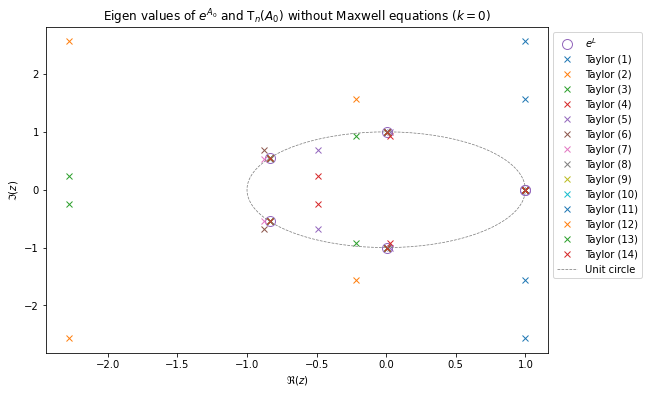
\includegraphics[width=\textwidth]{\localPath/figures/approx_evA0T5.png}
%     \caption{Les valeurs propres de $e^{A_0}$ et de $T_5(A_0)$}
%   \end{subfigure}
%   \begin{subfigure}{.5\textwidth}
%     \centering
%     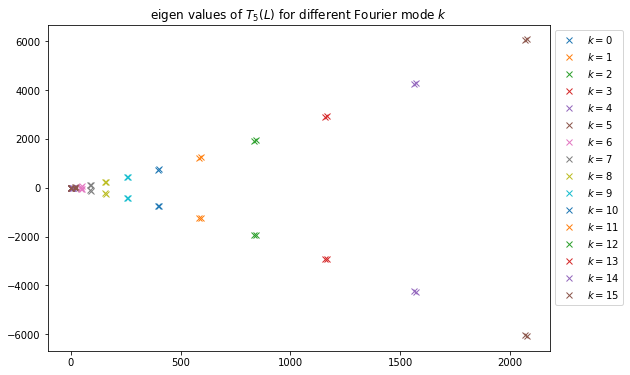
\includegraphics[width=\textwidth]{\localPath/figures/approx_evAkT5.png}
%     \caption{Les valeurs propres de $e^{A}$ et de $T_5(A)$ pour différentes valeurs de $k\in[\![0,15]\!]$, par symétrie on obtient aussi celles pour $k<0$}
%   \end{subfigure}
%   \caption{Valeurs propres de $e^{A}$ et de $T_5(A)$ pour $k=0$ (sans les équations de Maxwell) à gauche, et pour différentes valeurs de $k\in[\![0,15]\!]$ à droite.}
% \end{figure}

\begin{figure}
  \begin{subfigure}{.5\textwidth}
    \centering
    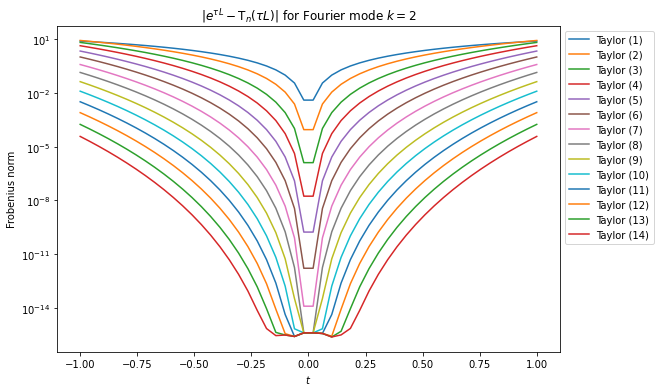
\includegraphics[width=\textwidth]{\localPath/figures/approx_errortA2T.png}
    \caption{L'erreur absolue locale $\|e^{tA}-T_p(tA)\|$ pour le mode de Fourier $k=2$}
  \end{subfigure}
  \begin{subfigure}{.5\textwidth}
    \centering
    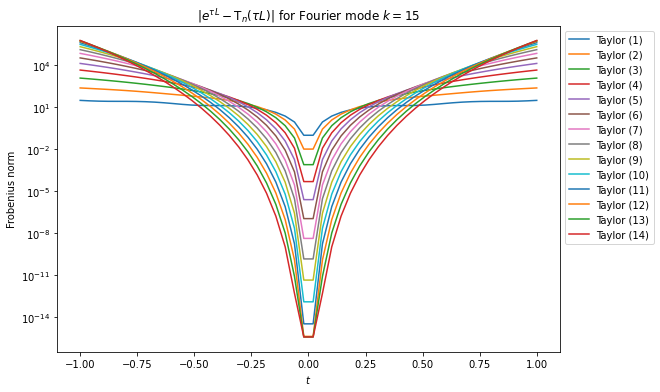
\includegraphics[width=\textwidth]{\localPath/figures/approx_errortA15T.png}
    \caption{L'erreur absolue locale $\|e^{tA}-T_p(tA)\|$ pour le mode de Fourier $k=15$}
  \end{subfigure}
  \caption{Erreur absolue locale $\|e^{tA}-T_p(tA)\|$ pour deux modes de Fourier $k=2$ à gauche et $k=15$ à droite.}
  \label{fig:taylor:error}
\end{figure}

\subsection{Approximant de Padé}
%--------------------------------------------------------------------

Pour approcher une fonction, au lieu d'utiliser un polynôme comme dans le cadre des séries des développement limités, il est possible de construire une fraction rationnelle. L'approximant de Padé de la fonction exponentielle est la meilleure approximation de la fonction exponentielle par une fraction rationnelle et est définie par :
$$
  \begin{aligned}
    h_{p,q}(x) &= \sum_{i=0}^p \frac{\frac{p!}{(p-i)!}}{\frac{(p+q)!}{(p+q-i)!}}\frac{x^i}{i!} \\
    k_{p,q}(x) &= \sum_{j=0}^q (-1)^j \frac{\frac{q!}{(q-j)!}}{\frac{(p+q)!}{(p+q-j)!}} \frac{x^j}{j!}
  \end{aligned}
$$

$$
  P_{p,q}(x) = \frac{h_{p,q}(x)}{k_{p,q}(x)} \approx e^x
$$

Pour utiliser cet approximant de Padé, qui est une fraction rationnelle, avec des matrices il faut utiliser la définition suivante :

$$
  e^M \approx P_{p,q}(M) = h_{p,q}(M)\cdot\left(k_{p,q}(M)\right)^{-1}
$$

L'introduction d'une fraction rationnelle permet de préserver certaines propriétés comme le fait que $P_{p,p}(-z) = \frac{1}{P_{p,p}(z)}$. Nous regardons les valeurs propres de $P_{2,2}(A)$, pour les modes de Fourier $\kappa\in[\![0,15]\!]$ sur la figure~\ref{fig:ev:P22}, et l'on remarque que, contrairement à la troncature de la série de Taylor, le module des valeurs propres est 1.

%\begin{figure}
%  \centering
%  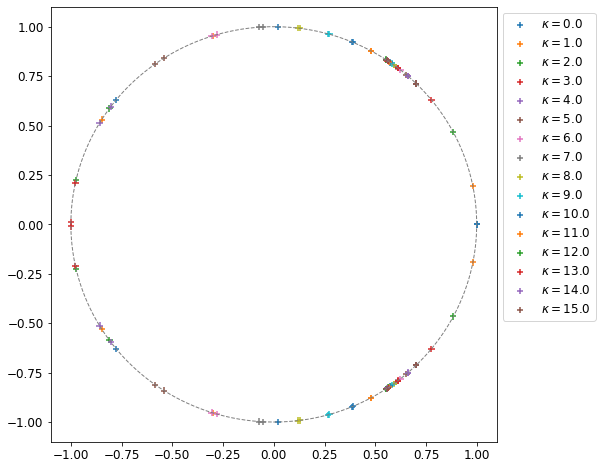
\includegraphics[width=0.5\textwidth]{\localPath/figures/ev_P22.png}
%  \caption{Valeurs propres de $P_{2,2}(A)$ pour différentes fréquences $\kappa\in[\![0,15]\!]$. Les valeurs propres des modes de Fourier négatifs, sont obtenues par parité.}
%  \label{fig:ev:P22}
%\end{figure}

% \begin{figure}
%   \begin{subfigure}{.5\textwidth}
%     \centering
%     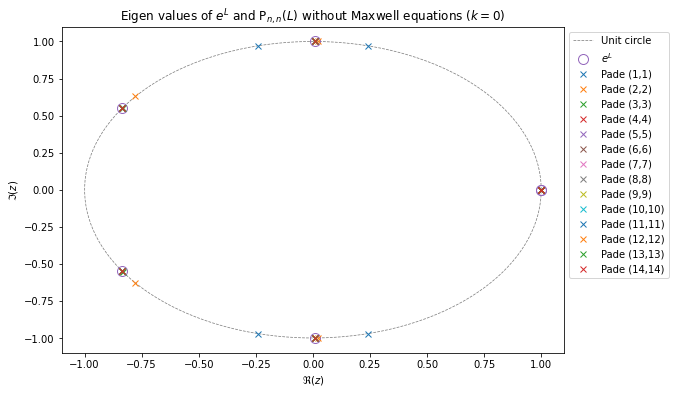
\includegraphics[width=\textwidth]{\localPath/figures/approx_evA0P.png}
%     \caption{Les valeurs propres de $e^{A_0}$ et de $P_{n,n}(A_0)$}
%   \end{subfigure}
%   \begin{subfigure}{.5\textwidth}
%     \centering
%     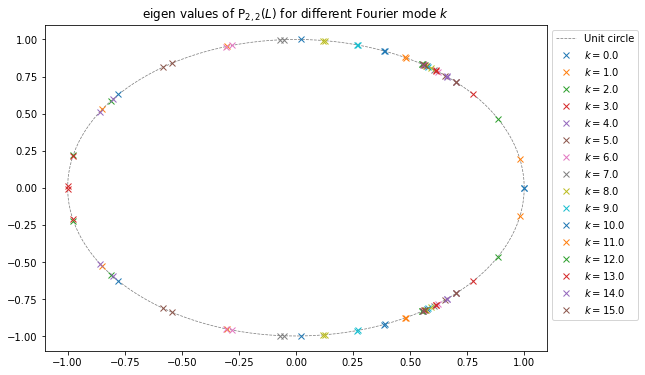
\includegraphics[width=\textwidth]{\localPath/figures/approx_evAkP22.png}
%     \caption{Les valeurs propres de $e^{A}$ et de $P_{2,2}(A)$ pour différentes valeurs de $k\in[\![0,15]\!]$, par symétrie on obtient aussi celles pour $k<0$}
%   \end{subfigure}
%   \caption{Valeurs propres de $e^{A}$ et de $P_{n,n}(A)$ pour $k=0$ (sans les équations de Maxwell) à gauche, et pour différentes valeurs de $k\in[\![0,15]\!]$ à droite.}
%   \label{fig:evAP22}
% \end{figure}

\begin{figure}
  \begin{subfigure}{.5\textwidth}
    \centering
    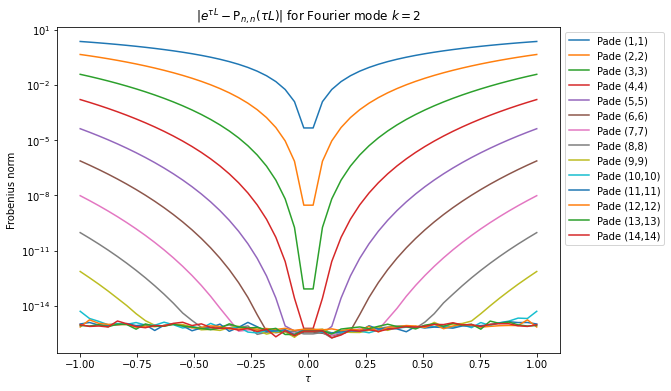
\includegraphics[width=\textwidth]{\localPath/figures/approx_errortA2P.png}
    \caption{L'erreur absolue locale $\|e^{tA}-P_{p,p}(tA)\|$ pour le mode de Fourier $\kappa=2$}
  \end{subfigure}
  \begin{subfigure}{.5\textwidth}
    \centering
    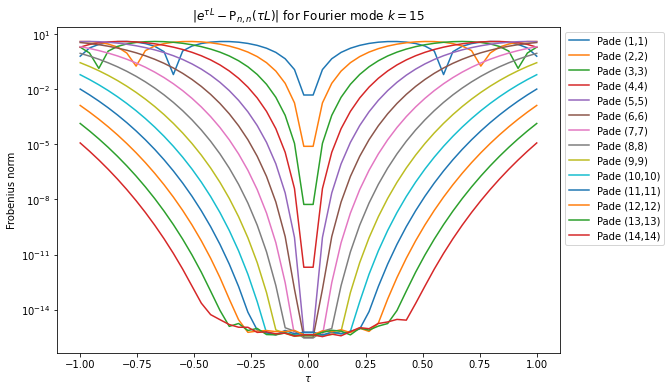
\includegraphics[width=\textwidth]{\localPath/figures/approx_errortA15P.png}
    \caption{L'erreur absolue locale $\|e^{tA}-P_{p,p}(tA)\|$ pour le mode de Fourier $\kappa=15$}
  \end{subfigure}
  \caption{Erreur absolue locale $\|e^{tA}-P_{p,p}(tA)\|$ pour deux modes de Fourier $\kappa=2$ à gauche et $\kappa=15$ à droite.}
\end{figure}

\begin{figure}
  \centering
  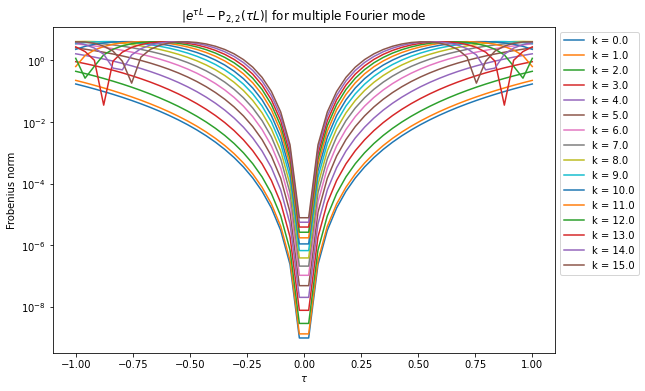
\includegraphics[width=0.75\textwidth]{\localPath/figures/approx_errortAkP22.png}
  \caption{L'erreur absolue locale $\|e^{tA}-P_{2,2}(tA)\|$ pour différents mode de Fourier.}
\end{figure}


\subsection{Test sur un modèle jouet}
%--------------------------------------------------------------------

Nous souhaitons mettre en place cette stratégie d'approximation de la partie linéaire d'une méthode de Lawson sur une première équation qui nous servira de \emph{toy model} :
$$
  \partial_t u = a\partial_x u + b\partial_y u
$$
où $u(t,x,y)$ est une fonction à valeurs réelles, $(x,y)\in[-2,2]\times[-2,2]$, $t\geq0$, $a,b\in\mathbb{R}$ donnés, et $u(t=0,x,y)=u_0(x,y)$ donné. On sait que la solution au temps $t$ est donnée par :
$$
  u(t,x,y) = u_0(x-at,y-bt).
$$
On souhaite résoudre cette équation par une méthode spectrale dans la direction $y$ (partie linéaire de la méthode de Lawson), une méthode WENO5 dans la direction $x$ (partie non-linéaire), et une méthode LRK($s$,$n$) en temps (méthode de Lawson d'ordre $n$ à $s$ étages). Nous obtenons donc l'équation :
$$
  \partial_t \hat{u} = L\hat{u} + N(\hat{u}),\quad u(t=0,x,y) = u_0(x,y)
$$
avec $L = i\kappa b$ et, $N:\hat{u}\mapsto\widehat{a\partial_xu}$. À partir des résultats du chapitre~\ref{chap1}, on peut calculer l'erreur du schéma en linéarisant la partie non-linéaire :
$$
  u^{n+1} = e^{\Delta tL}\sum_{i=0}^{n}\frac{\Delta t^iN^i}{i!}u^n = e^{\Delta t (L+N)}u^n + \order{\Delta t^{n+1}}
$$
ce qui nous permet de dire que la partie linéaire est résolue exactement, et que la partie non-linéaire est d'ordre 3. Il est également possible de vouloir approcher l'exponentielle de la partie linéaire $e^{\Delta tL}$ avec une troncature de la série de Taylor ou un approximant de Padé :
$$
  \begin{aligned}
    u^{n+1} =& T_m(\Delta tL)\sum_{i=0}^{n}\frac{\Delta t^iN^i}{i!}u^n     & & \text{pour la série de Taylor d'ordre $m$} \\
    u^{n+1} =& P_{p,q}(\Delta tL)\sum_{i=0}^{n}\frac{\Delta t^iN^i}{i!}u^n & & \text{pour l'approximant de Padé d'ordre $(p,q)$}
  \end{aligned}
$$
avec $T_m(\Delta tL) = e^{\Delta tL}+\order{\Delta t^m}$ et $P_{p,q}(\Delta tL) = e^{\Delta tL}+\order{\Delta t^{p+q}}$. Ce qui nous permet d'écrire :
$$
  u^{n+1} = e^{\Delta t (L+N)}u^n + \order{\Delta t^r} + \order{\Delta t^{n+1}}
$$
avec $r=m$ pour la troncature de la série de Taylor, ou $r=p+q$ pour l'approximant de Padé. Ainsi l'erreur en temps du schéma, approché par une méthode d'interpolation de la partie linéaire, est une contribution de deux termes, et l'ordre en temps de la méthode est $\min(r,n)$.

Il est possible de retrouver ce résultat numériquement en comparant les différentes méthodes et en mesurant l'erreur effectuée pour différentes valeurs de pas de temps $\Delta t$ et ainsi mesure l'ordre en temps de la méthode. Pour cela on choisit le schéma LRK(3,3) induit par la méthode SSP RK(3,3) de Shu-Osher, on se munit d'une discrétisation de $243$ points par direction, de plusieurs valeurs de pas de temps $\Delta t\in[0.00158,0.02370]$. La simulation s'effectue jusqu'au temps final $T_f=0.07111$ avec les vitesses $a=1.0$ et $b=0.75$. On regarde l'erreur, par rapport à notre solution de référence en norme 1 :
$$
  e_1 = \| u(t,x,y) - u_0(x-at,y-bt) \|_1 \approx \sum_{i,j}|u^n_{i,j}-u_0(x_i-at,y_j-bt)|\Delta x\Delta y,
$$
ce qui nous permet de tracer, sur la figure~\ref{fig:lrk33ref} l'erreur pour la méthode de référence avec un calcul exact de l'exponentielle de la partie linéaire, ainsi qu'avec une troncature de la série de Taylor d'ordre 4, ordre supérieur à celui de la méthode de Lawson, et un approximant de Padé d'ordre $(2,2)$ (équivalent à un ordre 4), aussi supérieur à l'ordre de la méthode de Lawson, on retrouve bien dans ces cas là l'ordre 3 de la méthode LRK(3,3). La figure~\ref{fig:lrk33taylor} représente l'ordre pour différentes troncatures de la série de Taylor, on remarque que pour des ordres inférieurs à l'ordre de la méthode de Lawson, on mesure l'ordre de la méthode de Taylor. La figure~\ref{fig:lrk33pade} quant à elle, représente l'ordre pour différents approximants de Padé, on retrouve les mêmes résultats avec une constante d'erreur plus faible.

\begin{figure}
  \centering
  \begin{subfigure}{.45\textwidth}
    \centering
    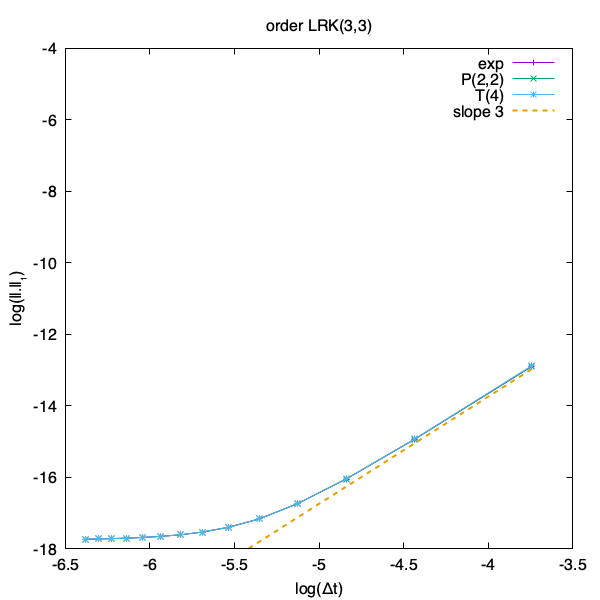
\includegraphics[width=\textwidth]{\localPath/figures/order_lrk33ref.png}
    \caption{Ordre en temps de la méthode LRK(3,3) associée à exponentielle, la série de Taylor d'ordre 4, et l'approximant Padé d'ordre $(2,2)$.}
    \label{fig:lrk33ref}
  \end{subfigure}
  \begin{subfigure}{.45\textwidth}
    \centering
    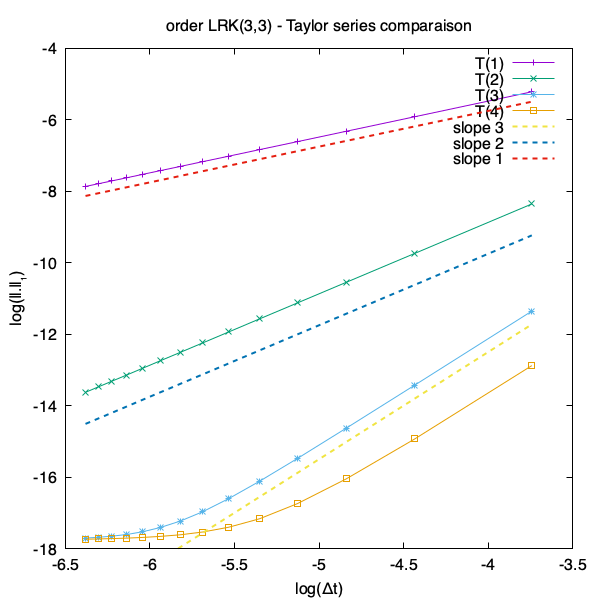
\includegraphics[width=\textwidth]{\localPath/figures/order_lrk33taylor.png}
    \caption{Ordre en temps de la méthode LRK(3,3) associée à la série de Taylor d'ordre 1 à 4.\\ }
    \label{fig:lrk33taylor}
  \end{subfigure}
  \begin{subfigure}{.45\textwidth}
    \centering
    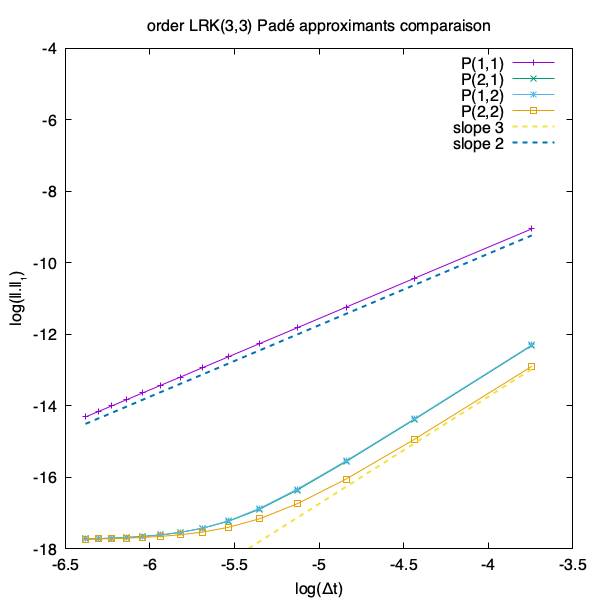
\includegraphics[width=\textwidth]{\localPath/figures/order_lrk33pade.png}
    \caption{Ordre en temps de la méthode LRK(3,3) associée à l'approximant Padé d'ordre $(1,1)$, $(2,1)$, $(1,2)$, et $(2,2)$.}
    \label{fig:lrk33pade}
  \end{subfigure}
  \caption{Ordre en temps de la méthode LRK(3,3) où l'exponentielle de la partie linéaire est approchée par différentes méthodes, série de Taylor ou approximant de Padé de différents ordre. La solution de référence à gauche, le test avec différentes séries de Taylor à droite, et avec différents approximant de Padé en bas.}
  \label{fig:3:order}
\end{figure}
